\documentclass[tikz]{standalone}
\usepackage{mathpazo}

\usetikzlibrary{calc}

\usetikzlibrary{arrows.meta}

\usetikzlibrary{decorations.markings}

\begin{document}


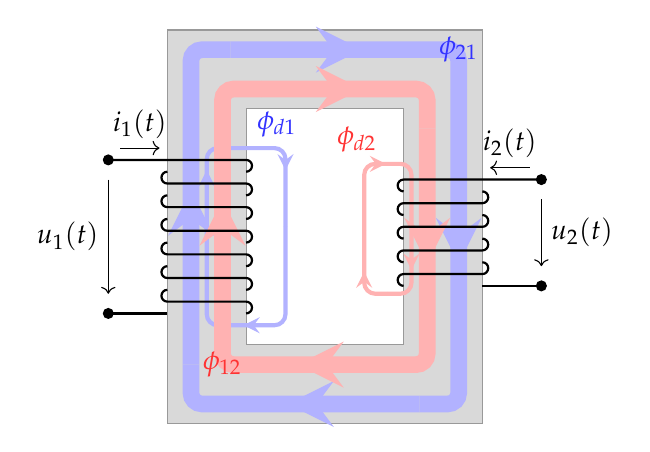
\begin{tikzpicture}
\draw[black!40, fill = black!15] (0,0) rectangle (4,5);
\draw[black!40, fill = white] (1,1) rectangle (3,4);

%% FLUJOS
\tikzset{flow/.style = {line width = 6pt,
    rounded corners,
    decoration={%
      markings,
      mark=at position .5 with {\arrow{stealth}}},postaction={decorate}}}

% Flujo de bobina 1 a bobina 2
\tikzset{flow1/.style = {flow, blue!30}}
\draw[flow1] (.3,.75) coordinate (A1) |- ++(.5,4) coordinate (B1);
\draw[flow1] (B1) -| node[blue!80, midway] {$\phi_{21}$} ++(2.9,-.5) coordinate (C1);
\draw[flow1] (C1) |- ++(-.5,-4) coordinate (D1);
\draw[flow1] (D1) -| (A1);


% Flujo de dispersión de la bobina 1
\tikzset{flowd1/.style = {flow, line width = 1.5pt, blue!30}}
\draw[flowd1] (.5,2.5) coordinate (Ad1) |- ++(.5,1) coordinate (Bd1);
\draw[flowd1] (Bd1) node[blue!80, above right] {$\phi_{d1}$} -|  ++(.5,-1) coordinate (Cd1);
\draw[flowd1] (Cd1) |-  ++(-.75,-1.25) -| (Ad1);

% Flujo de bobina 2 a bobina 1
\tikzset{flow2/.style = {flow, red!30}}
\draw[flow2] (.7,1) coordinate (A2) |- ++(.5,3.25) coordinate (B2);
\draw[flow2] (B2) -| ++(2.1,-.5) coordinate (C2);
\draw[flow2] (C2) |- ++(-.5,-3) coordinate (D2);
\draw[flow2] (D2) -| node[midway, red!80] {$\phi_{12}$} (A2);

% Flujo de dispersión de la bobina 2
\tikzset{flowd2/.style = {flow, line width = 1.5pt, red!30}}
\draw[flowd2] (3.1, 2.5) coordinate (Ad2) |- ++(-.3,-.85) coordinate (Bd2);
\draw[flowd2] (Bd2) -|  ++(-.3,.8) coordinate (Cd2);
\draw[flowd2] (Cd2) |-  ++(.3,.85) node[red!80, above left] {$\phi_{d2}$} -| (Ad2);

%% BOBINAS

%Bobina 1
\begin{scope}[shift={(0,3.5)}]
  \coordinate (in) at (-.75, -1.5mm);
  \coordinate (out) at (-.75, -21mm);
  \draw[thick] (in)--(0,-1.5mm)--++(0:1cm) arc[start angle=90, delta angle=-180, radius=.75mm]; 
  \foreach \i in {1,...,6}
  {\draw[thick] (0,-3mm * \i) arc[start angle=90, delta angle=180, radius=.75mm]--++(0:1cm) arc[start angle=90, delta angle=-180, radius=.75mm]; }
  \draw[thick] (out) -- ++(.75, 0) ++(0:2.5mm);
  \fill (in) circle (2pt);
  \fill (out) circle (2pt);
  \draw[->]($(in) + (0,-.25)$) -- ($(out) + (0,.25)$) node[midway, left]{$u_1(t)$};
  \draw[->]($(in) + (.15, .15)$) -- ++(.5, 0) node[midway, above]{$i_1(t)$};
\end{scope}

%Bobina 2
\begin{scope}[shift={(4,3.25)}, xscale=-1]
  \coordinate (in) at (-.75, -1.5mm);
  \coordinate (out) at (-.75, -15mm);
  \draw[thick] (in)--(0,-1.5mm)--++(0:1cm) arc[start angle=90, delta angle=-180, radius=.75mm]; 
  \foreach \i in {1,...,4}
  {\draw[thick] (0,-3mm * \i) arc[start angle=90, delta angle=180, radius=.75mm]--++(0:1cm) arc[start angle=90, delta angle=-180, radius=.75mm]; }
  \draw[thick] (out) -- ++(.75, 0) ++(0:2.5mm);
  \fill (in) circle (2pt);
  \fill (out) circle (2pt);
  \draw[->]($(in) + (0,-.25)$) -- ($(out) + (0,.25)$) node[midway, right]{$u_2(t)$};
  \draw[->]($(in) + (.15, .15)$) -- ++(.5, 0) node[midway, above]{$i_2(t)$};
\end{scope}


\end{tikzpicture}
\end{document}